Compare $y^2 = 4x$ to the general equation
\begin{align}
    ax^2 + 2bxy + cy^2 + 2dx + 2ey + f = 0
\end{align}
a=b=e=0, d=-2, c=1, f=0
\begin{align}
  \vec{V} = \myvec{a & b \\ b & c} = \myvec{0 & 0 \\ 0 & 1}\\
  \vec{u} = \myvec{d \\ e} = \myvec{-2 \\ 0}\\
  \mydet{V} = \mydet{0 & 0 \\ 0 & 1} = 0
\end{align}
 $\implies$ The curve is a parabola. Since
\begin{align}
     \vec{Vp_{1}} = 0\\
    \implies \vec{p_{1}} = \myvec{1 \\ 0}
\end{align}
The slope of the given line is m. The direction vector $\vec{m}$ would be
\begin{align}
   \vec{m} = \myvec{1 \\ m}\\
   \vec{m}^T\vec{n} = 0\\
   \vec{n} = \myvec{m \\ -1}
\end{align}
Equation for point of contact for the parabola is 
\begin{align}
    \myvec{\vec{u}^T + \kappa \vec{n}^T \\ \vec{V}}\vec{q} = \myvec{-f \\ \kappa \vec{n} - \vec{u}}\\
   where, \kappa = \frac{\vec{p}_{1}^T \vec{u}}{\vec{p}_{1}^T \vec{n}} = - \frac{2}{m}
\end{align}
Substitute the values to get
\begin{align}
   \myvec{-4 & \frac{2}{m} \\ 0 & 0 \\ 0 & 1}\vec{q} = \myvec{0 \\ 0 \\ \frac{2}{m}} \label{eq:solutions/3/2/21/eq:3}
\end{align}
Solving for $\vec{q}$ by removing the zero row and represent Eq \eqref{eq:solutions/3/2/21/eq:3} as augmented matrix and convert it into echelon form
\begin{align}
\implies \myvec{-4 & \frac{2}{m} & 0 \\ 0 & 1 & \frac{2}{m}}
\xleftrightarrow{R_1\leftarrow \frac{-R_1}{4}}
\myvec{1 & -\frac{1}{2m} & 0 \\ 0 & 1 & \frac{2}{m}}\\
\xleftrightarrow{R_1\leftarrow R_1 + \frac{1}{2m}R_2}
\myvec{1 & 0 & \frac{1}{m^2} \\ 0 & 1 & \frac{2}{m}}\\
\end{align}
The point of contact is $\myvec{\frac{1}{m^2} \\ \frac{2}{m}}$. Substitute this in Eq \eqref{eq:solutions/3/2/21/eq: 1}
\begin{align}
    \myvec{-m & 1}\myvec{\frac{1}{m^2} \\ \frac{2}{m}} = 1\\
    -\frac{1}{m} + \frac{2}{m} = 1\\
    \frac{1}{m} = 1\\
    \implies m = 1
\end{align}
\begin{figure}[!ht]
\centering
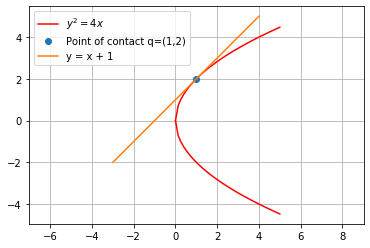
\includegraphics[width=\columnwidth]{./solutions/3/2/21/A5.png}
\caption{}
\label{eq:solutions/3/2/21/Fig:1}
\end{figure}
